\documentclass[10pt,twoside,slovak,a4paper]{article}

\usepackage[slovak]{babel}
\usepackage[IL2]{fontenc}
\usepackage[utf8]{inputenc}
\usepackage{graphicx}
\usepackage{url}
\usepackage{hyperref}
\usepackage{cite}

\pagestyle{headings}

\title{Metódy detekcie prania špinavých peňazí v kryptomenových
transakciách: prehľad súčasného stavu\thanks{Semestrálny projekt v predmete
Metódy inžinierskej práce, ak. rok 2026/27, vedenie: Meno Priezvisko}}

\author{Oleksandr Komarenko\\[2pt]
	{\small Slovenská technická univerzita v Bratislave}\\
	{\small Fakulta informatiky a informačných technológií}\\
	{\small \texttt{xkomarenko@stuba.sk}}
	}

\date{\small 3. október 2026}

\begin{document}

\maketitle

\begin{abstract}
Verejné blockchainy zaznamenávajú každú transakciu trvalo a sprístupňujú ju
komukoľvek, totožnosť účastníkov však zostáva skrytá za pseudonymnými adresami.
Táto kombinácia otvorenosti a anonymity vytvára prostredie, v ktorom možno
presúvať prostriedky nelegálneho pôvodu a zároveň zahladzovať ich stopu.
Článok prináša prehľad súčasného stavu v oblasti detekcie prania špinavých
peňazí v kryptomenových transakciách. Zhrňujeme typológiu praktík používaných
na zastieranie pôvodu prostriedkov, porovnávame skupiny prístupov k ich
odhaľovaniu --- od heuristík na zhlukovanie adries cez analýzu transakčného
grafu až po metódy strojového učenia --- a venujeme sa dostupným datasetom
a metrikám, ktorými sa tieto prístupy hodnotia. V závere identifikujeme
otvorené problémy, medzi ktoré patrí najmä nedostatok overených označených
údajov, vysvetliteľnosť rozhodnutí a napätie medzi dohľadom a ochranou
súkromia.
\end{abstract}

% ---------------------------------------------------------------
% POZNÁMKA PRE TÍM: zatiaľ len štruktúra. Text dopĺňame po častiach,
% každú zmenu commitujeme vo vetve predbeznaVerzia.
% ---------------------------------------------------------------

\section{Úvod} \label{uvod}

% Čím sa zaoberáme a prečo. Motivácia, rozsah problému, štruktúra článku.


\section{Východiská} \label{vychodiska}

% Základné pojmy: blockchain, transakcia, adresa, pseudonymita,
% zmenáreň, mixér. Definície podľa iných autorov a naše vymedzenie.


\section{Pranie špinavých peňazí v kryptomenovom prostredí} \label{typologia}

% Fázy prania, typológia praktík, odkaz na regulačný rámec (AMLD, MiCA, FATF).


\section{Prístupy k detekcii} \label{pristupy}

% Hlavná časť prehľadu. Porovnanie skupín metód.

\subsection{Heuristiky na zhlukovanie adries} \label{pristupy:heuristiky}

\subsection{Analýza transakčného grafu} \label{pristupy:graf}

\subsection{Metódy strojového učenia} \label{pristupy:ml}


\section{Datasety a hodnotenie} \label{hodnotenie}

% Dostupné datasety, metriky, problém nevyvážených tried a chýbajúcich označení.

% --- Miesto pre tabuľku porovnania prístupov ---


\section{Otvorené problémy} \label{problemy}

% Čo zostáva nevyriešené: označené údaje, vysvetliteľnosť, falošné poplachy,
% ochrana súkromia, rýchly vývoj techník zastierania.

% --- Miesto pre diagram; po exporte z UMLetu odkomentovať ---
%\begin{figure*}[tbh]
%\centering
%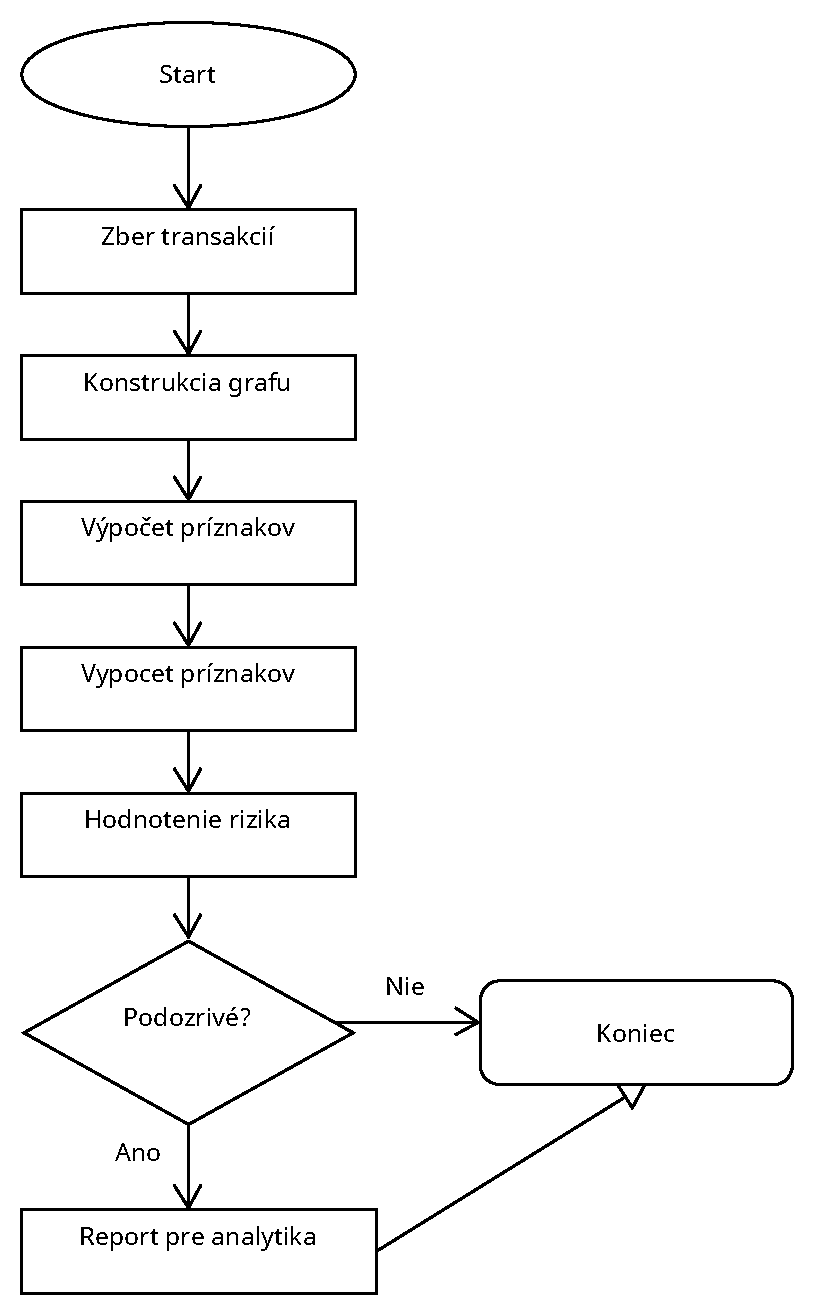
\includegraphics[scale=1.0]{diagramy/diagram.pdf}
%\caption{Schéma typického reťazca zastierania pôvodu prostriedkov.}
%\label{f:retazec}
%\end{figure*}


\section{Záver} \label{zaver}

% O čom je článok, k čomu prispieva, čo zostáva otvorené.


\bibliography{literatura}
\bibliographystyle{plain}

\end{document}